\documentclass[10pt,a4paper]{article}
\usepackage[margin=2.1cm,top=2.0cm,bottom=2.2cm]{geometry}
\usepackage[T1]{fontenc}
\usepackage{mathpazo}
\usepackage{amsmath,amssymb,graphicx,booktabs,xcolor,caption,enumitem,microtype,tikz,tabularx}
\usetikzlibrary{arrows.meta,positioning,calc}
\usepackage[colorlinks=true,linkcolor=black!70!blue,citecolor=black!70!blue,urlcolor=black!60!blue]{hyperref}
\captionsetup{font=small,labelfont=bf,width=0.96\textwidth}
\setlist{nosep,leftmargin=1.4em}
\setlength{\parskip}{3pt}
\definecolor{ink2}{HTML}{52514E}
\definecolor{blueA}{HTML}{2A78D6}
\definecolor{orangeA}{HTML}{EB6834}
\definecolor{aquaA}{HTML}{1BAF7A}
\definecolor{boxbg}{HTML}{F4F4F1}
\newcommand{\ts}{\tilde s}
\newcommand{\Tavg}{T_{\mathrm{avg}}}
\newcommand{\Trelax}{T_{\mathrm{relax}}}
\newcommand{\Fz}{F_0}
\graphicspath{{../results/}}

\title{\vspace{-1.2cm}\Large\bfseries A Kerr microring resonator as the policy of a reinforcement-learning agent\\[2pt]
\normalsize\mdseries Notes on the simulations, the results and what they do and do not show}
\author{\normalsize Pavel Dolgirev \quad\textcolor{ink2}{\small (repository \texttt{aion-optical-RL}; 22 September 2026)}}
\date{}

\begin{document}
\maketitle
\vspace{-0.9cm}

\noindent\colorbox{boxbg}{\parbox{\dimexpr\textwidth-2\fboxsep}{\small
\textbf{Summary.}\; We asked whether an optical microring resonator---a passive, chip-scale Kerr-nonlinear cavity that is
already a workhorse of frequency-comb research---can serve as the \emph{policy} of a reinforcement-learning agent: the
observation of the environment is written into the light that drives the ring, the ring's output spectrum is read by
photodetectors, and the only trainable element is a single linear layer of a few dozen weights that turns detected line
powers into an action.  In simulations of the standard Lugiato--Lefever model, trained with an unmodified proximal-policy-optimisation
(PPO) loop in which the ring's own output is what the agent acts on:
(i) the optical policy balances the CartPole benchmark in every run (score 500/500 on 64 test episodes,
36 trainable weights), in every dynamical regime of the ring that admits a single-valued response---a chaotic frequency comb,
a stationary Turing-roll pattern, a single soliton and a ring without pattern formation; (ii) on a task that a linear policy provably cannot solve, swinging
up a pendulum with a three-level torque, the pattern-free ring with 54 trainable weights matches an
899-weight neural-network policy on three seeds, because the Kerr nonlinearity supplies the product features
(angular velocity $\times$ orientation) that the task needs, and on LunarLander (8 inputs, 4 actions) the same ring with
eight tones and 136 weights lands as reliably as a 1668-weight network where the linear policy again fails; (iii) the ring's physics dictates the design: chaos makes the
time-averaged spectrum a single-valued function of the input (at the price of a quantifiable ``chaos noise''), a
translation symmetry of the ring forbids the naive sign-encoding of inputs, and pattern-forming states (rolls, solitons)
tolerate only weak inputs and act as linear transducers.  One decision costs $\sim$30--150\,ns of light in a ring of
$Q = 3\times10^6$.  The nonlinearity exploited so far is mild (5--10\,\% of the feature variance), and an explicit quadratic
feature map performs as well; the result is an existence proof and a design guide, not yet evidence of an optical advantage.}}

\section{Why this question}
Reinforcement learning (RL) is dominated by the cost of evaluating a policy network millions of times.  Physical
substrates whose natural dynamics compute a nonlinear map---``physical reservoirs''---have been used as feature
generators for classification and time-series prediction, and in one hardware demonstration an optoelectronic delay-line
reservoir with 600 trained output weights solved CartPole and MountainCar by Q-learning at MHz rates
\cite{ref:sci_rep_2022}.  Kerr microresonators are attractive substrates because a single chip-scale ring transforms a
few input tones into hundreds of comb lines through a strong, fast $\chi^{(3)}$ nonlinearity; chaotic and stationary microcombs
have been proposed as reservoirs \cite{ref:prr_2025,ref:nanoph_2025}.  What has not been established is whether such a device can
sit inside an \emph{on-policy} RL loop as the nonlinear stage of the policy itself---and, more basically, which of the ring's very
different dynamical states (chaos, rolls, solitons, none) is a usable feature map for a memoryless controller.  These notes
answer both questions in simulation.

\section{The optical policy}

\begin{figure}[h]
\centering
\resizebox{\textwidth}{!}{%
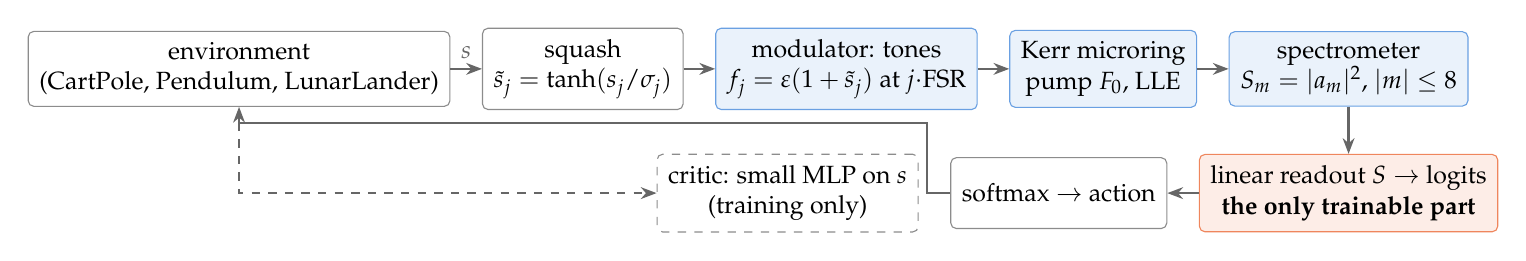
\begin{tikzpicture}[font=\small, node distance=4mm,
  box/.style={draw=black!45, rounded corners=2pt, fill=white, minimum height=9mm, align=center, inner sep=4pt},
  opt/.style={box, fill=blueA!10, draw=blueA!70},
  train/.style={box, fill=orangeA!12, draw=orangeA!80},
  arr/.style={-{Stealth[length=2mm]}, thick, black!60}]
\node[box] (env) {environment\\(CartPole, Pendulum, LunarLander)};
\node[box, right=of env] (enc) {squash\\$\ts_j=\tanh(s_j/\sigma_j)$};
\node[opt, right=of enc] (mod) {modulator: tones\\$f_j=\varepsilon(1+\ts_j)$ at $j\cdot$FSR};
\node[opt, right=of mod] (ring) {Kerr microring\\pump $\Fz$, LLE};
\node[opt, right=of ring] (det) {spectrometer\\$S_m=|a_m|^2$, $|m|\le 8$};
\node[train, below=6mm of det] (lin) {linear readout $S\to$ logits\\ \textbf{the only trainable part}};
\node[box, left=of lin] (act) {softmax $\to$ action};
\node[box, dashed, left=of act] (crit) {critic: small MLP on $s$\\(training only)};
\draw[arr] (env) -- node[above]{$s$} (enc);
\draw[arr] (enc) -- (mod);
\draw[arr] (mod) -- (ring);
\draw[arr] (ring) -- (det);
\draw[arr] (det) -- (lin);
\draw[arr] (lin) -- (act);
\draw[arr] (act.west) -- ++(-3mm,0) |- ($(env.south)+(0,-2mm)$) -- (env.south);
\draw[arr, dashed] (env.south) ++(0,-2mm) |- (crit.west);
\end{tikzpicture}}
\caption{The optical policy.  Blue boxes are optics (nothing in them is trained); the orange box holds the 36
(CartPole), 54 (Pendulum) or 136 (LunarLander) trainable weights.  PPO trains the readout and the critic; the ring is
simulated by the Lugiato--Lefever equation.}
\label{fig:pipeline}
\end{figure}

\paragraph{Encoding.}  Each component $s_j$ of the observation ($d=4$ for CartPole, $3$ for the pendulum, $8$ for LunarLander) is squashed to
$\ts_j\in[-1,1]$ and written as the amplitude of a sub-band tone that drives cavity mode $m=j$, i.e.\ amplitude modulation
of the pump laser at $j$ times the free spectral range:
\[
F(\varphi)=\Fz+\sum_{j=1}^{d}\varepsilon\,(1+\ts_j)\,e^{\,i j\varphi}\qquad(\text{tones weaker than the pump: }\varepsilon\le 0.32\,\Fz).
\]
\paragraph{Ring.}  The intracavity field obeys the dimensionless Lugiato--Lefever equation (LLE),
$\partial_t\psi=-(1+i\Delta)\psi+i d_2\partial_\varphi^2\psi+i|\psi|^2\psi+F(\varphi)$, with time in units of the photon
lifetime $2/\kappa$, detuning $\Delta$ and dispersion $d_2$; $\psi=\sum_m a_m e^{im\varphi}$ and $|a_m|^2$ is the power in
comb line $m$.  The simulator is a PyTorch port of the JAX solver of the companion repository \texttt{rc-chaotic-comb}, which
reproduces \cite{ref:prr_2025} (agreement between the two solvers $4\times10^{-13}$); it is extended to multi-tone drives and
batched over 64 rings.
\paragraph{Detection and readout.}  The policy sees the powers of the $4d+1$ lines $|m|\le 2d$ (17 for CartPole; a filter bank and photodiodes), standardised
with fixed calibration statistics, and turns them into action logits with one linear layer.  Nothing else about the
optics is trained.  A separate small network (the critic, 4-128-1) estimates the value of the raw state; it is a training aid and is
discarded afterwards.
\paragraph{Training.}  The PPO implementation is the one previously validated with a neural-network policy (clipped ratio,
GAE, 20 epochs per buffer of 2048 steps, Adam $10^{-2}$).  Two things change because the policy is a physical device: 64
environments run in parallel, each wired to its own persistent ring; and the buffer stores the features the ring
\emph{actually produced} when the action was taken, so that the later gradient steps evaluate $\pi(a\,|\,S_t)$ on the
same optical output that acted---a chaotic ring asked twice about the same state answers differently.

\section{Which state of the ring is a usable feature map}
A memoryless policy needs the map $\ts\to S$ to be single-valued (no dependence on what the ring did before), fast, strong
enough to rise above the detector, and---if the ring is to do more than transduce---nonlinear.  Driven Kerr rings offer
four qualitatively different states; we tested all four (Fig.~\ref{fig:regimes}).

\begin{figure}[t]
\centering
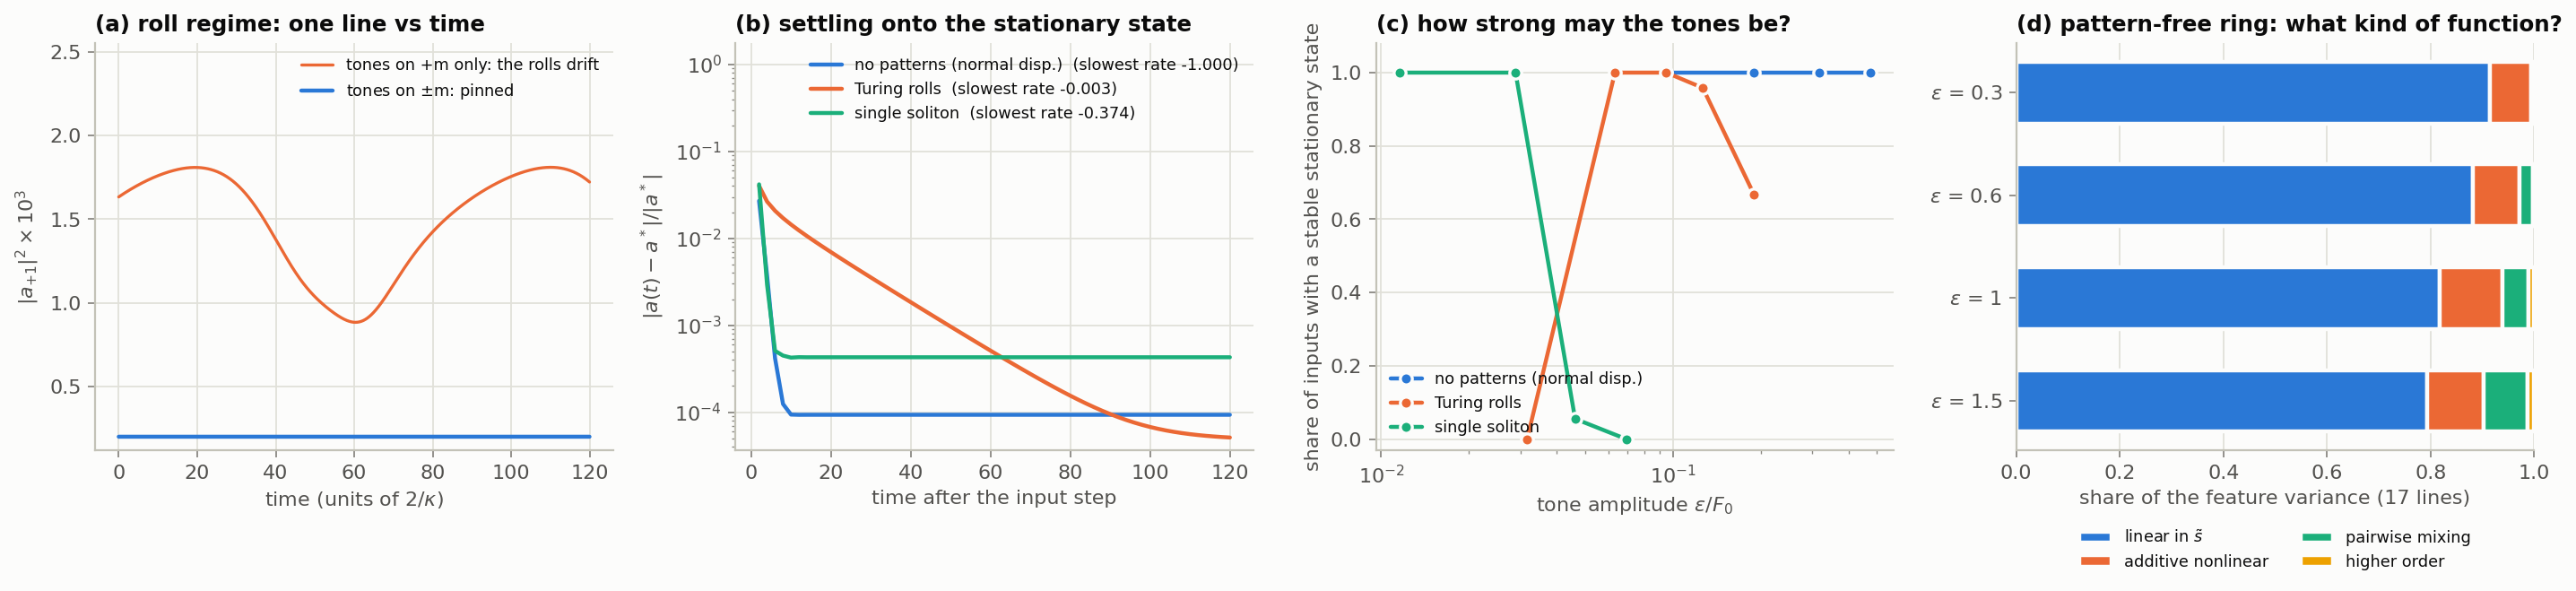
\includegraphics[width=\textwidth]{characterization/04_beyond_chaos.png}
\caption{Ordered states of the ring as feature maps.  (a)~Tones on modes $+m$ only break the reflection symmetry of the
ring and make a roll pattern drift; tones on $\pm m$ (plain amplitude modulation) pin it.  (b)~Settling after an input
step: the pattern-free ring relaxes at the photon-decay rate, a soliton somewhat slower, a roll pattern has a soft
positional mode (rate $-0.003$).  (c)~Share of inputs for which the followed branch is linearly stable: rolls tolerate
tones up to $\varepsilon\approx0.1\Fz$, a soliton only $\approx0.03\Fz$, the pattern-free ring everything tried.
(d)~Decomposition of the feature variance of the pattern-free ring into parts linear in $\ts$, additive-nonlinear, pairwise
mixing $\ts_i\ts_j$ and higher order, versus tone amplitude.}
\label{fig:regimes}
\end{figure}

\begin{description}[style=unboxed,leftmargin=0pt,itemsep=2pt]
\item[Chaotic comb (anomalous dispersion, pump well above threshold).]  The instantaneous spectrum is useless---it
depends on the chaotic trajectory---but the comb is ergodic, so its \emph{time average} is a single-valued smooth function of
the drive.  The price is chaos noise: averaging over a window $\Tavg$ leaves a relative fluctuation $c_v\sqrt{2\tau_c/\Tavg}$
with $c_v\approx0.85$ and a correlation time $\tau_c\approx0.5$ lifetimes, i.e.\ 17\,\% per line at $\Tavg=25$ (measured and
predicted curves coincide, Appendix Fig.~\ref{fig:avg}).  Two findings shaped the design.  First, the operating point of
\cite{ref:prr_2025} is only marginally chaotic under a constant pump (largest Lyapunov exponent $+0.09$; long-time averages differ by
70\,\% between realisations); at pump power $\Fz^2=10$ the exponent is $+0.55$ and the averages agree.  Second, a symmetry
forbids the obvious encoding $f_j=\varepsilon\ts_j$: the LLE is invariant under $\varphi\to\varphi+\varphi_0$, which
multiplies every tone by $e^{im\varphi_0}$ and changes no line power, so the time-averaged spectrum depends on the tones only
through invariants such as $|f_j|^2$; a signed encoding is blind to the sign of every input at leading order, and
$\varphi_0=\pi$ makes ``cart and pole to the left'' \emph{exactly} indistinguishable from ``to the right''.  The offset
encoding $f_j=\varepsilon(1+\ts_j)$ removes the degeneracy; trained with the signed encoding the agent never exceeds a
return of 102.
\item[Ring without pattern formation (normal dispersion, monostable detuning).]  No modulational instability, hence no
chaos and no patterns: for every input there is one stable stationary state, reached at the photon-decay rate
(a few lifetimes), with zero noise.  The response is nevertheless nonlinear (Fig.~\ref{fig:regimes}d): at
$\varepsilon=0.32\Fz$, 82\,\% of the feature variance is linear in $\ts$, 12\,\% additive-nonlinear, 5\,\% pairwise mixing.
We simulate this regime directly in the stationary limit, by Newton continuation of the fixed point from the ring's previous
state; a physical ring is in that limit whenever the control interval exceeds a few lifetimes.
\item[Turing rolls and single solitons.]  Both are stationary only if the tones are placed symmetrically on $\pm m$
(Fig.~\ref{fig:regimes}a).  A roll pattern has a soft positional mode and coexisting roll numbers, and loses its branch
above $\varepsilon\approx0.1\Fz$; a soliton breathes or nucleates further solitons above $\varepsilon\approx0.03\Fz$.
At the tone amplitudes they tolerate their response is essentially linear: they are transducers, not computers.
\end{description}

\noindent For the chaotic comb we also measured directly how nonlinear the response to the tones is (Appendix
Fig.~\ref{fig:nonlin}): a single tone produces the driven line and its four-wave-mixing idler in strict linear
response up to $\varepsilon\approx0.8\Fz$; genuine mixing between two inputs (a sum-frequency line, non-additive response)
appears above $\varepsilon\approx0.3\Fz$.  With the four-tone encoding, pairwise mixing carries 7\,\% of the idler-line signal
at $\varepsilon=0.19\Fz$ and 24\,\% at $0.32\Fz$.  ``Weaker than the pump but nonlinear'' therefore means
$\varepsilon\approx0.2$--$0.3\Fz$; the defaults are $\varepsilon=0.19\Fz$ (chaos) and $0.32\Fz$ (stationary).

\section{Results}

\begin{figure}[t]
\centering
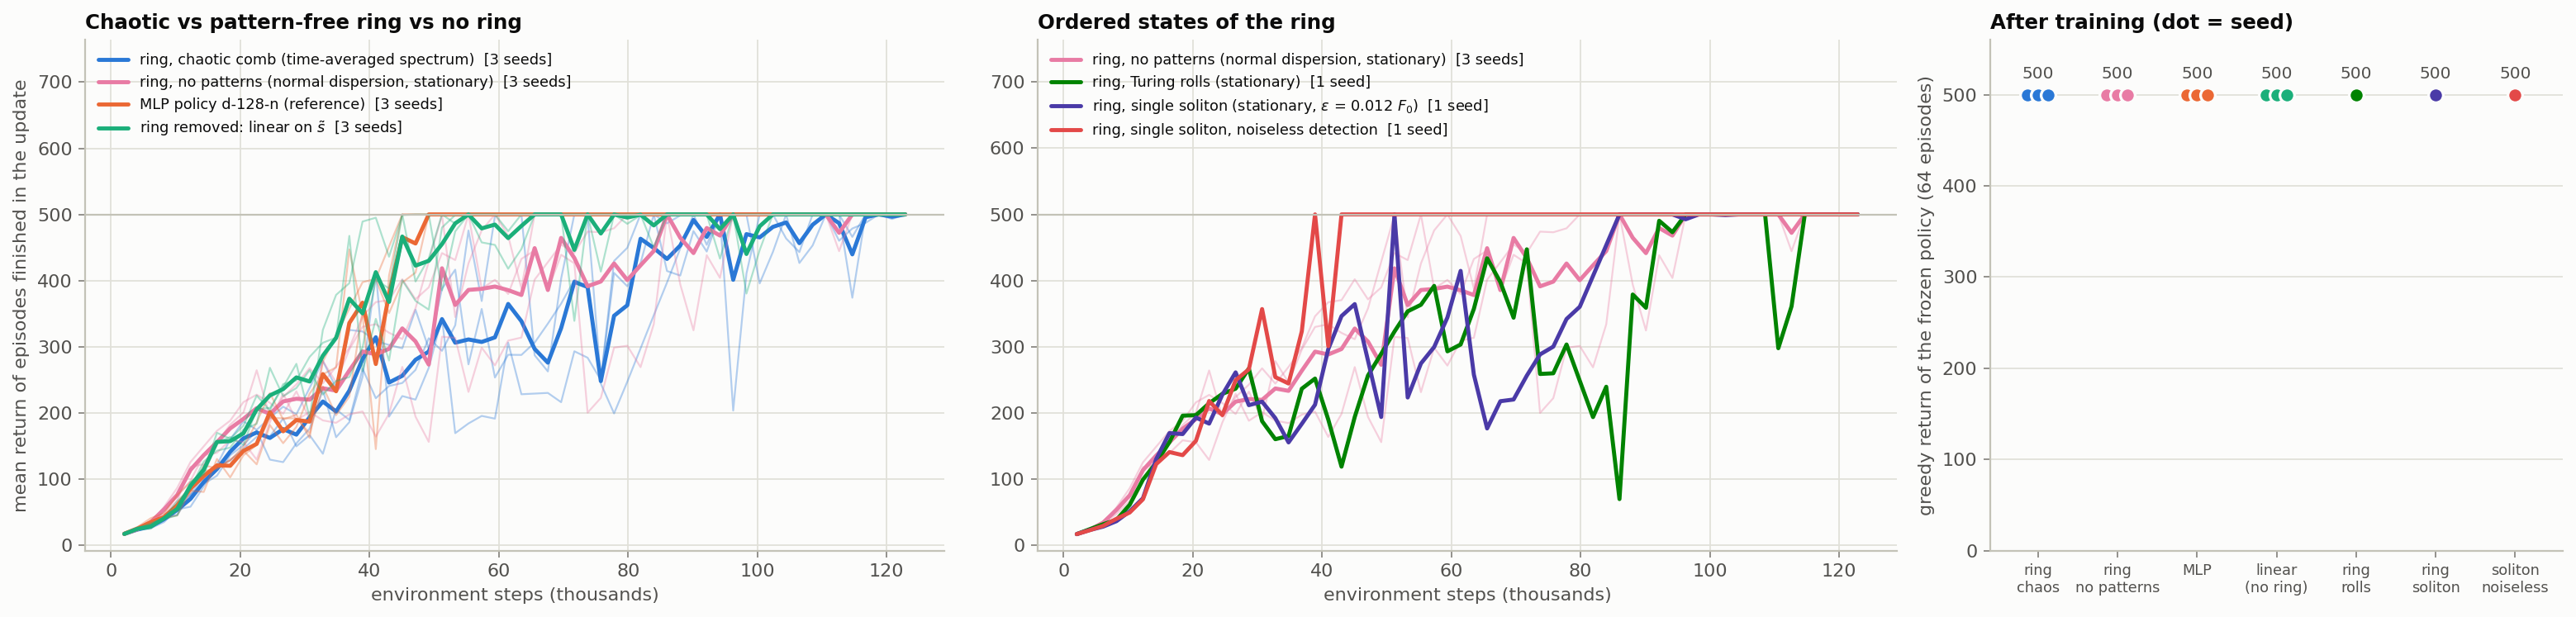
\includegraphics[width=\textwidth]{ppo/CartPole/comparison.png}
\caption{CartPole-v1.  Left: learning curves (mean return of the episodes finished in each update; thin lines are single
seeds, bold the seed average) for the chaotic and the pattern-free ring against the same PPO loop with a neural-network
policy and with the ring removed (a linear layer applied to the same squashed inputs).  Middle: the ordered states.
Right: greedy return of the frozen final policies over 64 fresh episodes.}
\label{fig:cartpole}
\end{figure}

\paragraph{CartPole: every regime works.}  Table~\ref{tab:cartpole} and Fig.~\ref{fig:cartpole}.  The chaotic ring
(36 weights) reaches a training return of 475 after 55--90k environment steps against 39--51k without the ring---the price of
17\,\% feature noise---and its frozen policy scores the maximum 500 on all 64 test episodes for each of three seeds.
The pattern-free ring, which has no noise, learns as fast as the ring-free baseline (51--78k) and also scores 500/500 on all
seeds.  The roll ring at its weak $\varepsilon$ solves the task too (500/500, one seed), consistent with its acting as a
linear transducer; the soliton ring solves it as well once the tones are weak enough for its branch never to be lost ($\varepsilon=0.012\Fz$: 500/500 with or without a 1\,\% detector error, learning as fast as the ring-free policy), whereas at $\varepsilon=0.03\Fz$, where the branch is lost in a few percent of the decisions, PPO does not learn at all and the run was stopped.  The
trained optical readouts are reproducible across seeds although each run sees different chaotic trajectories, and they are
interpretable: projected through the ring's measured small-signal response, the chaotic-ring readout implements gains of
about $(2.1, 2.5, 3.6, 8.8)$ on $(x,\dot x,\theta,\dot\theta)$, against $(1.7, 3.7, 3.2, 7.1)$ for the linear policy trained
without the ring (Appendix Fig.~\ref{fig:readout})---the same controller, routed through the comb lines.

\begin{table}[h]
\centering\small
\caption{CartPole-v1 (maximum return 500).  ``Steps to 475'': environment steps at which the mean training return first
reached 475, per seed.  ``Frozen'': greedy return of the final policy over 64 fresh episodes, per seed.}
\label{tab:cartpole}
\begin{tabular}{lrll}
\toprule
policy & weights & steps to 475 & frozen \\
\midrule
ring, chaotic comb ($\varepsilon=0.19\Fz$, $\Tavg=25$) & 36 & 90k / 55k / 84k & 500 / 500 / 500 \\
ring, no patterns (stationary, $\varepsilon=0.32\Fz$) & 36 & 55k / 51k / 78k & 500 / 500 / 500 \\
ring, Turing rolls (stationary, $\varepsilon=0.06\Fz$) & 36 & 92k & 500 \\
ring, single soliton (stationary, $\varepsilon=0.012\Fz$) & 36 & 51k & 500 \\
neural network 4-128-2 & 898 & 49k / 45k / 45k & 500 / 500 / 500 \\
ring removed: linear layer on $\ts$ & 10 & 45k / 51k / 39k & 500 / 500 / 500 \\
\bottomrule
\end{tabular}
\end{table}

\paragraph{A task that needs the nonlinearity: pendulum swing-up.}  In Pendulum-v1 the agent must swing a pendulum from
hanging to upright with a torque too weak to lift it directly, here restricted to three levels $\{-2,0,+2\}$; the return
is a negative cost (0 is perfect, a passive pendulum scores about $-1200$).  A linear policy cannot both pump energy at the
bottom (torque $\propto+\dot\theta$) and brake at the top (torque $\propto-\dot\theta$); the smallest sufficient policy needs
a product of the angular velocity with a function of the orientation.  Table~\ref{tab:pendulum} and Fig.~\ref{fig:pendulum}:
the linear policy indeed fails on every seed (mean frozen return $-718$ to $-1038$), an explicit quadratic feature map
solves the task ($-147$ to $-159$), and so does the pattern-free ring with 54 weights ($-196$ to $-252$, against $-173$ to
$-239$ for the neural network)---its median episode ($-130$) equals that of the quadratic and neural-network policies, while a
few episodes from one corner of the state space (2--4 of 64 per seed) fail to swing up and lower its mean.  The policy maps (Fig.~\ref{fig:pendulum}, bottom) show what the readout
learned: the energy-pumping switching line $u\propto\mathrm{sign}[\dot\theta\, g(\theta)]$ that a linear policy cannot draw.  The
chaotic ring learns the same structure but more slowly and with a noisier boundary (mean $-428$, median $-392$ after 410k
steps): here the 17\,\% chaos noise on the features costs real performance.

\begin{table}[h]
\centering\footnotesize
\caption{Pendulum-v1 with three torque levels (0 is perfect; $\approx-1200$ is doing nothing).  Both rings use
$\varepsilon=0.32\Fz$ (the chaotic one with $\Tavg=25$).  Frozen policies, 64 fresh episodes, per seed: mean return, median
return and the share of episodes that end better than $-300$.}
\label{tab:pendulum}
\setlength{\tabcolsep}{4pt}
\begin{tabular}{lrlll}
\toprule
policy & weights & frozen, mean & median & share $>-300$ \\
\midrule
ring, no patterns (stationary) & 54 & $-252$ / $-196$ / $-206$ & $-130$ / $-131$ / $-131$ & 0.86 / 0.94 / 0.89 \\
ring, chaotic comb (410k steps) & 54 & $-428$ & $-392$ & 0.45 \\
neural network 3-128-3 & 899 & $-173$ / $-205$ / $-239$ & $-131$ / $-249$ / $-251$ & 0.88 / 0.88 / 0.80 \\
linear layer on $\ts$ (no ring) & 12 & $-718$ / $-1038$ / $-759$ & $-670$ / $-1001$ / $-687$ & 0.41 / 0.02 / 0.31 \\
explicit $\ts_i\ts_j$ features (no ring) & 30 & $-159$ / $-147$ / $-153$ & $-130$ / $-130$ / $-130$ & 0.94 / 1.00 / 0.97 \\
\bottomrule
\end{tabular}
\end{table}

\begin{figure}[t]
\centering
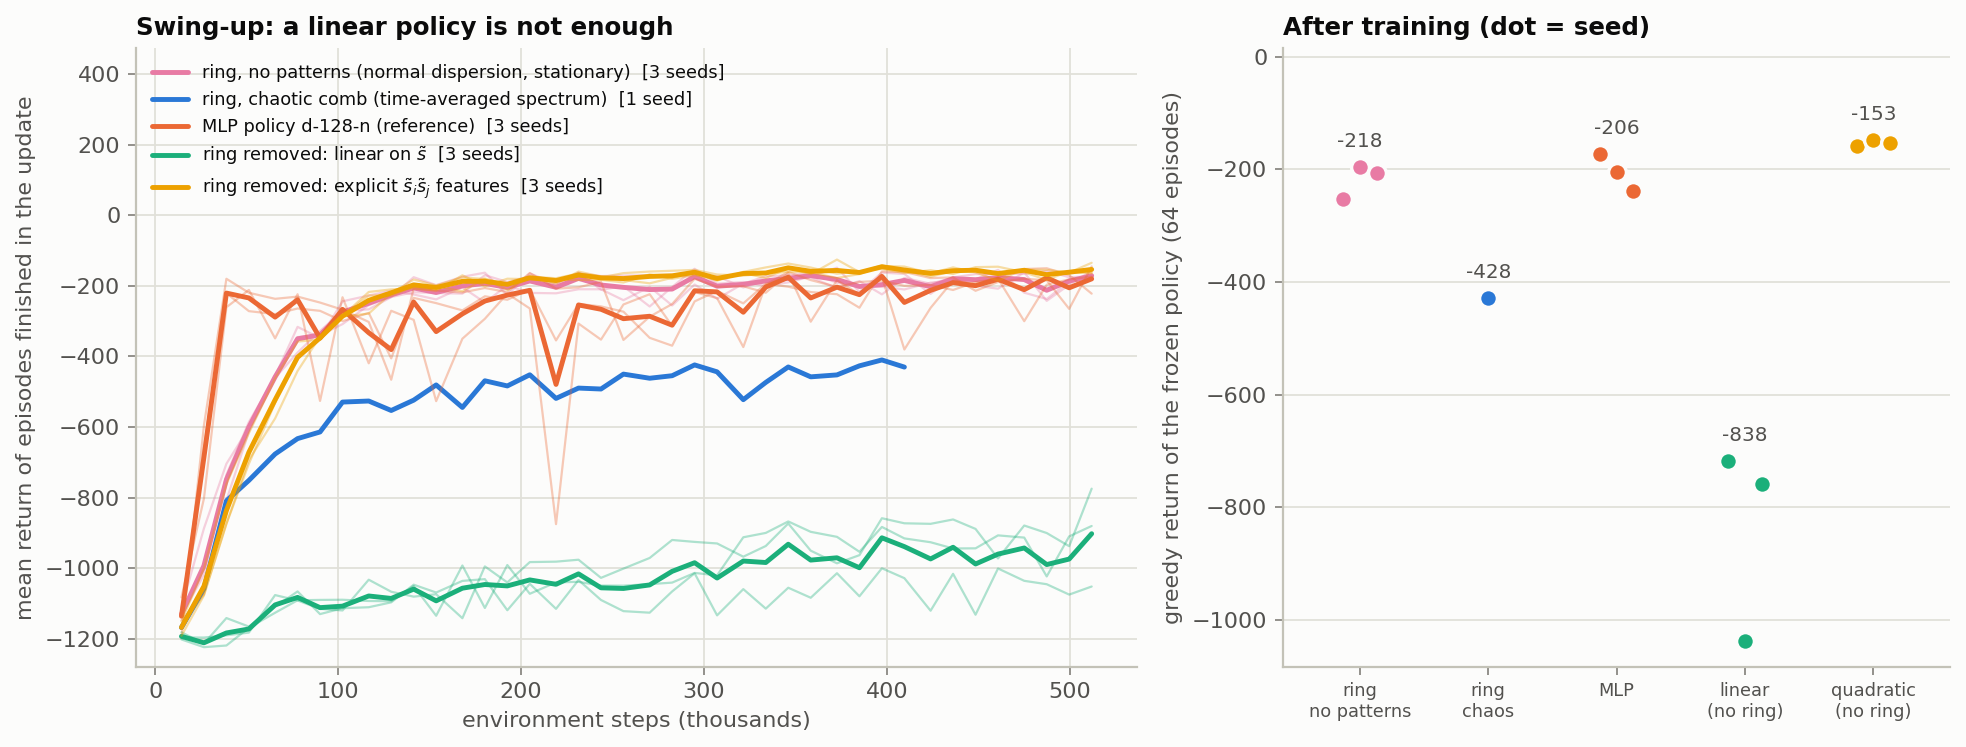
\includegraphics[width=0.99\textwidth]{ppo/Pendulum/comparison.png}\\[4pt]
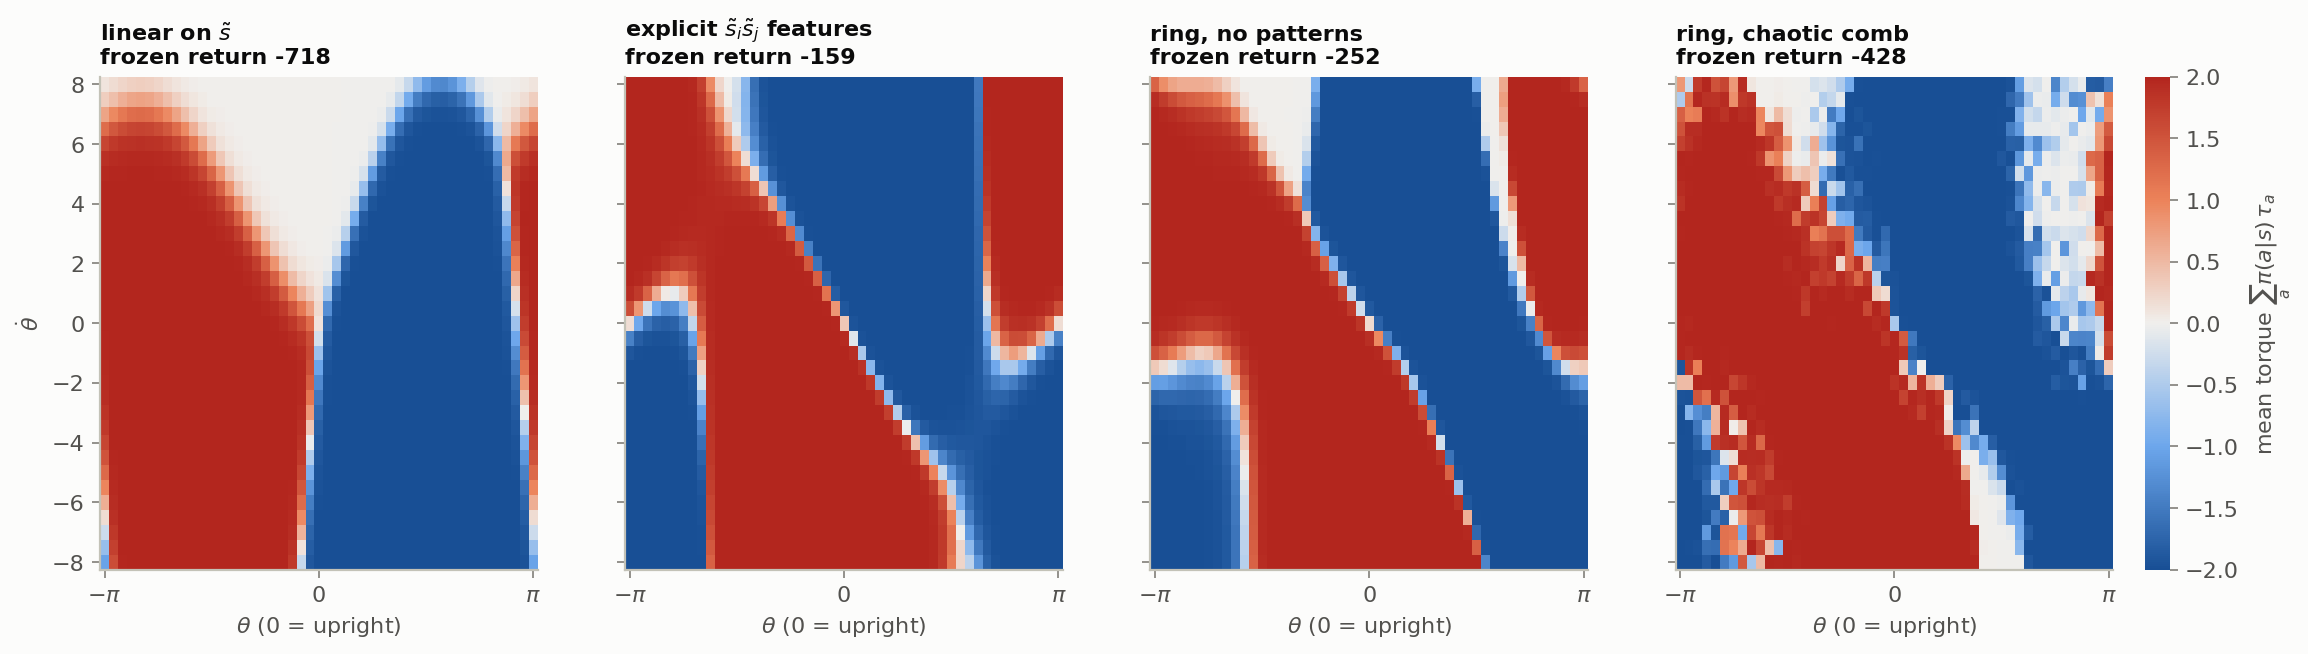
\includegraphics[width=0.99\textwidth]{ppo/Pendulum/policy_map.png}
\caption{Pendulum swing-up.  Top: learning curves and frozen returns.  Bottom: the trained policies as maps of the mean
torque over the $(\theta,\dot\theta)$ plane ($\theta=0$ upright).  The linear policy can only draw a boundary that is
a single line in $(\cos\theta,\sin\theta,\dot\theta)$; the quadratic map and the rings draw the switching curve that pumps
energy into the swing and removes it near the top.}
\label{fig:pendulum}
\end{figure}

\paragraph{More inputs: LunarLander.}  LunarLander-v3 has eight inputs (position, velocity, angle, angular velocity and
two leg-contact flags) and four actions (do nothing, fire left, main or right engine); a landing scores $\gtrsim200$, a crash
$\approx-100$ or worse.  Each input drives its own comb line ($m=1\ldots8$) and the readout sees the 33 lines $|m|\le16$.
With eight tones the ring is driven harder and its response is more nonlinear than in the four-tone case (on the
eight-dimensional input cube: 56\,\% linear, 32\,\% additive-nonlinear, 8\,\% pairwise mixing, 5\,\% higher order at
$\varepsilon=0.32\Fz$), while every stationary state visited in 514k decisions remained stable and the branch had to be
re-prepared in 0.1\,\% of them.  Table~\ref{tab:lunar} and Fig.~\ref{fig:lunar}: the linear policy fails on every seed
(frozen mean 106 / 25 / 7), and the ring with 136 weights lands the module as reliably as the 1668-weight network and the
180-weight explicit quadratic map (263 / 254 against 267--274 and 255--271; 92--95\,\% of episodes above 200).

\begin{table}[h]
\centering\small
\caption{LunarLander-v3 (a landing scores $\gtrsim200$).  Frozen policies, 64 fresh episodes, per seed: mean return, median and
the share of episodes with return $\ge200$.  Ring: pattern-free stationary regime, eight tones at $\varepsilon=0.32\Fz$, 33 lines.}
\label{tab:lunar}
\begin{tabular}{lrlll}
\toprule
policy & weights & frozen, mean & median & share $\ge200$ \\
\midrule
ring, no patterns (stationary) & 136 & 263 / 254 & 271 / 265 & 0.95 / 0.92 \\
neural network 8-128-4 & 1668 & 267 / 271 / 274 & 276 / 284 / 280 & 0.92 / 0.95 / 0.97 \\
linear layer on $\ts$ (no ring) & 36 & 106 / 25 / 7 & 124 / $-11$ / $-11$ & 0.28 / 0.03 / 0.06 \\
explicit $\ts_i\ts_j$ features (no ring) & 180 & 271 / 255 / 268 & 276 / 271 / 272 & 0.97 / 0.81 / 0.98 \\
\bottomrule
\end{tabular}
\end{table}

\begin{figure}[t]
\centering
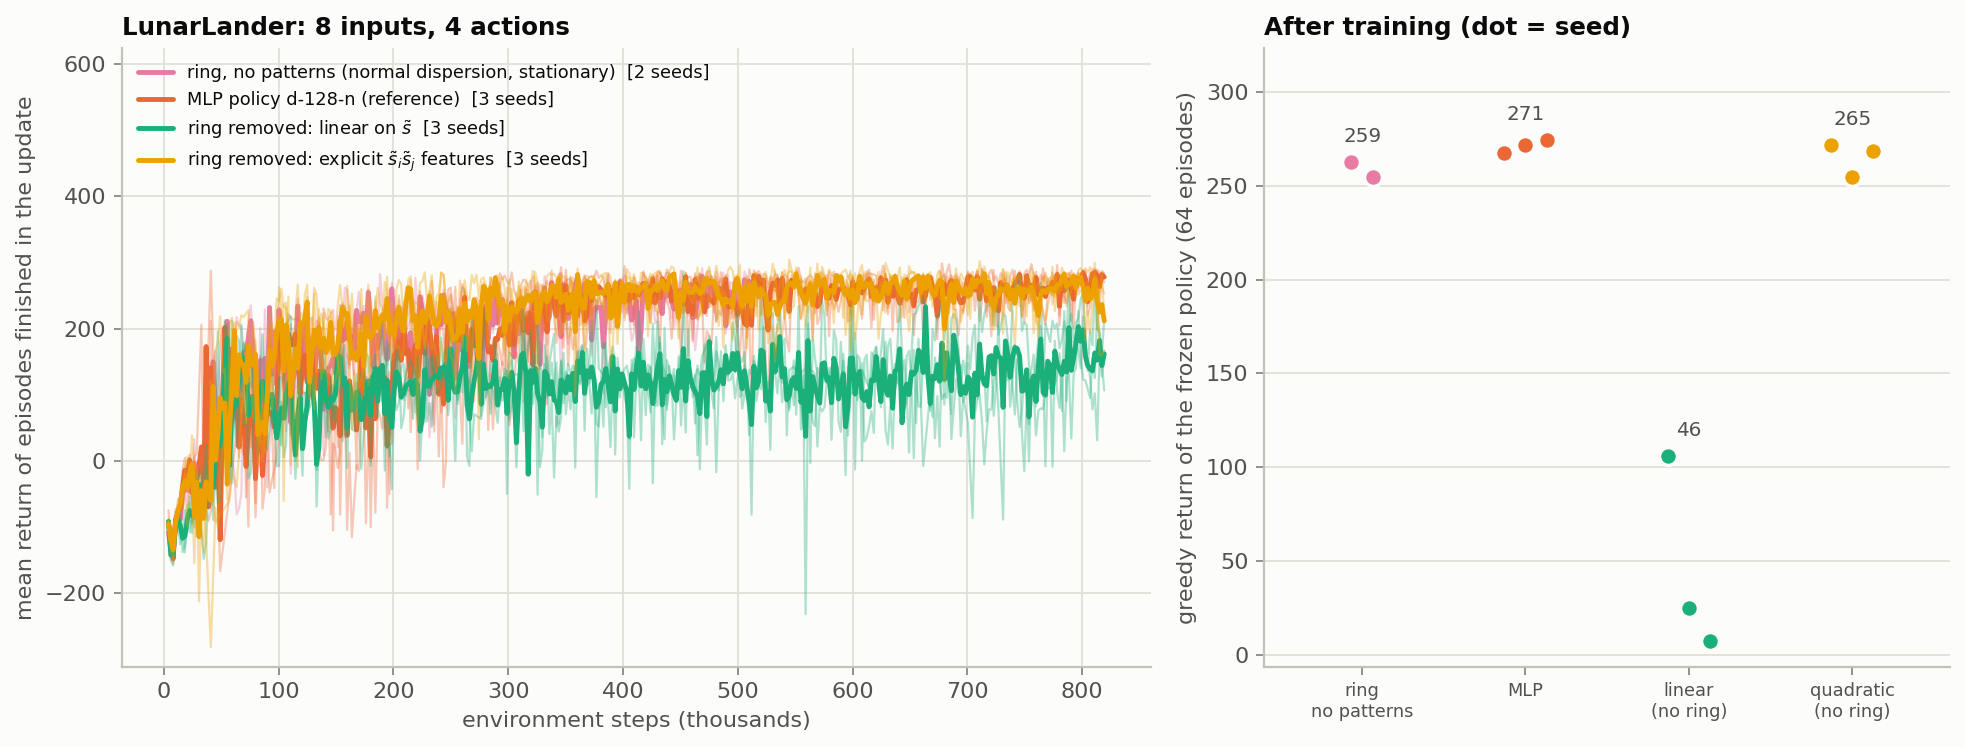
\includegraphics[width=0.99\textwidth]{ppo/LunarLander/comparison.png}
\caption{LunarLander-v3: learning curves (the ring runs were stopped after 512k steps, the baselines after 819k) and frozen
returns.}
\label{fig:lunar}
\end{figure}

\paragraph{What matters (ablations on the chaotic ring, CartPole).}  Appendix Fig.~\ref{fig:ablation}.  The signed
encoding fails, as the symmetry argument predicts.  Shorter averaging windows learn at a similar pace but the frozen policies
degrade ($\Tavg=5$: frozen 259/488/484; $\Tavg=10$: 393/474/498): with noisier features the readout does not learn the weak
cart-position feedback and the cart drifts off the track, a failure that the training curves hide because the ongoing
updates keep correcting it.  Reading all 128 lines instead of 17 (258 weights) works equally well; tone amplitudes
$\varepsilon=0.1$--$0.32\Fz$ all work.  White noise of similar magnitude added to the inputs of the ring-free linear policy does
\emph{not} slow its learning, so the chaotic ring's slower learning is not explained by feature noise alone; the readout
must also find the controller among many weakly informative, correlated lines.

\section{What this shows, and what it does not}
\begin{itemize}[itemsep=2pt]
\item \textbf{Shown.}  A Kerr microring can be the entire nonlinear stage of an RL policy and be trained in the loop with an
unmodified on-policy algorithm, with the optics' own (noisy, chaotic, or stationary) output as the agent's observation.
The physics constrains the design in ways that matter: developed chaos or a monostable ring is required for a
single-valued map, the encoding must respect the ring's translation symmetry, and pattern-forming states are too fragile
to compute with.  On swing-up and on LunarLander the ring's Kerr mixing provides the second-order features the tasks need,
with the trainable part reduced to 54 and 136 multiply--accumulates.
\item \textbf{Not shown.}  Any \emph{representational} advantage over a trivial digital feature map: an explicit quadratic
map does as well on every task, and the ring's nonlinear share of the features is 5--10\,\% with four tones and
$\approx45$\,\% with eight.  The tasks are toy benchmarks with 3--8 inputs.  Everything is simulation: the only noise is the chaos itself plus a 1\,\% detector error in the stationary
regime; laser phase noise, thermal drift of the resonance and detector bandwidth are not modelled.  Several rows rest on
one or two seeds.  Hyperparameters were chosen by hand from the characterisation, not optimised.
\end{itemize}

\section{Where an optical advantage could come from}
The processing in the ring is not ``at the optical frequency'': the ring can only follow its inputs on the scale of its
photon lifetime, $2/\kappa=5.5$\,ns for the $Q=3.3\times10^6$ device of \cite{ref:prr_2025}, so a decision costs 3--5
lifetimes $\approx20$--30\,ns in the stationary regime ($\gtrsim30$\,MHz) and $\Trelax+\Tavg=28$ lifetimes $\approx150$\,ns in
the chaotic one (6\,MHz).  A lower-$Q$ ring is faster but needs a stronger pump (the comb threshold scales as $1/Q^2$).
Training never differentiates through the ring---PPO treats the ring's output as the observation and trains the readout
digitally---so the same loop runs on hardware without a device model, and the ring is exercised at its decision rate during
the rollouts; training cost is dominated by environment interaction either way.  At \emph{inference} the nonlinear map is
done passively by the ring and the trained part is 36--136 multiply--accumulates on photodiode currents, within reach of an
analogue weighting network.  Two caveats and one prospect follow.  First, at these problem sizes digital electronics is
already at that speed: an 8-input quadratic policy is 44 features and 180 multiply--accumulates, one clock cycle on an
FPGA (5--10\,ns), and the pump laser ($\sim$100\,mW continuous wave for Si$_3$N$_4$ at this $Q$) costs $\sim$3\,nJ per decision
at 30\,MHz where 180 digital operations cost $\sim$0.2\,nJ---for a 4--8-input policy the optical route is at best a wash.
Second, in real-time control at 50\,Hz a frame is $3.6\times10^6$ lifetimes, so the chaos noise studied here would average
away entirely; the noise-limited regime is the one relevant to MHz-rate decisions or to massively batched policy
evaluation.  The prospect: the ring forms all pairwise four-wave-mixing products of its comb lines at once, so the cost of
an $N$-input quadratic map is independent of $N$ in the ring and grows as $N^2$ digitally---at $N\approx10^3$ inputs written
onto $10^3$ comb lines (an image-like observation) the digital map is $\sim5\times10^5$ operations per decision, microseconds
on an FPGA, against the same $\sim$30\,ns and pump power in the ring, and inputs that are already optical need no
converters.  Whether the ring's mixing products are the \emph{useful} features at that scale, with the signal per line
falling as the comb widens, is exactly what has not been shown.  A practical note: at the free spectral ranges of
microrings (10--1000\,GHz) the tones on modes $1\ldots d$ are not electro-optic sidebands of one laser but $d$ lasers on
neighbouring resonances, each intensity-modulated at the decision rate, plus the pump---standard telecom hardware whose
cost grows linearly with the number of inputs.

\section{Next steps}
(1) Tasks with many more inputs (low-resolution Atari frames written as 32--64 tones---one comb has room for them),
where the ring's $N$-independent cost could show, run at $\varepsilon\approx0.3\Fz$ where mixing terms are a quarter of the
signal, and with the intensity--intensity correlations $\langle|a_{m_1}|^2|a_{m_2}|^2\rangle$ of the
modified reservoir scheme as additional second-order features.  (2) Symmetric $\pm m$ tones with differential detection to
reject common-mode laser noise.  (3) Training the readout in situ by evolution strategies, which needs no gradients through
the optics and can fold the hardware noise into the search distribution.  (4) A hardware test: pump laser, one
intensity-modulated laser per input on neighbouring resonances, a Si$_3$N$_4$ ring, an arrayed-waveguide filter and 17--33 photodiodes.

\appendix
\section{Methods in brief}
\paragraph{Solver.}  Strang splitting with both sub-flows exact: the Kerr step is the phase rotation
$\psi\to\psi e^{i|\psi|^2\mathrm{d}t}$ and the linear step including the drive is solved mode by mode,
$a_m\to e^{L_m\mathrm{d}t}a_m+(e^{L_m\mathrm{d}t}-1)F_m/L_m$; $N=128$ modes, $\mathrm{d}t=0.01$ lifetimes (mean spectra identical to
$\mathrm{d}t=0.005$ within statistics).  Operating points: chaos $\Delta=1.76$, $d_2=0.0125$, $\Fz^2=10$; pattern-free
$\Delta=1$, $d_2=-0.0125$, $\Fz^2=10$; rolls $\Delta=0$, $d_2=0.0125$, $\Fz^2=2.5$; soliton $\Delta=3$, $d_2=0.0125$, $\Fz^2=3$.
The dispersion is 3.6 times that of \cite{ref:prr_2025} so that the chaotic comb fits in 128 modes; the LLE only
knows $d_2m^2$, so this is the same ring with the mode index rescaled by 1.9.
\paragraph{Stationary regimes.}  The fixed point $G(\psi)=0$ is found by a modified Newton iteration on the $2N\times2N$
real Jacobian (LU factorisation reused while the residual contracts), warm-started from the ring's previous state so that the
same branch is followed; input jumps larger than $0.25\varepsilon$ are sub-stepped.  The Jacobian spectrum gives the
linear stability of every state visited (all stable in the runs reported).  The continuation reproduces long-time
integration to $5\times10^{-5}$ and is about ten times cheaper.
\paragraph{Feature map.}  Chaos: hold the tones for $\Trelax=3$ (discarded) then $\Tavg=25$ lifetimes, sample the line
powers every 0.05; the ring state carries over between decisions.  Squashing scales $\sigma=(1,0.75,0.075,0.75)$ for
$(x,\dot x,\theta,\dot\theta)$, $(1,1,8)$ for $(\cos\theta,\sin\theta,\dot\theta)$ and $(0.6,0.8,0.8,0.8,0.5,0.6,1,1)$ for the
LunarLander state.  Features are standardised with mean
and standard deviation from a task-independent sweep of the inputs over $[-1,1]^d$ before training; the readout starts at zero
(uniform random policy).
\paragraph{PPO.}  64 environments $\times$ 32 steps per update, GAE $\lambda=0.95$, clip 0.2, 20 policy epochs and 20 critic
iterations per buffer, Adam $10^{-2}$ for both; $\gamma=0.99$ and 60 updates (123k steps) for CartPole, $\gamma=0.95$,
reward scaled by 0.1 and 250 updates (512k steps) for the pendulum (200 for the chaotic ring); $\gamma=0.99$, reward scaled
by 0.05, 400 updates (819k steps) for LunarLander (250 for the ring).  Frozen policies are evaluated
greedily (argmax) on 64 fresh episodes; for the rings the evaluation uses freshly prepared rings.  One CartPole run costs
$\approx$20 min of ring simulation on a laptop core (chaos) or 15 min (stationary); a pendulum run 65 min.

\section{Additional figures}
\begin{figure}[h]
\centering
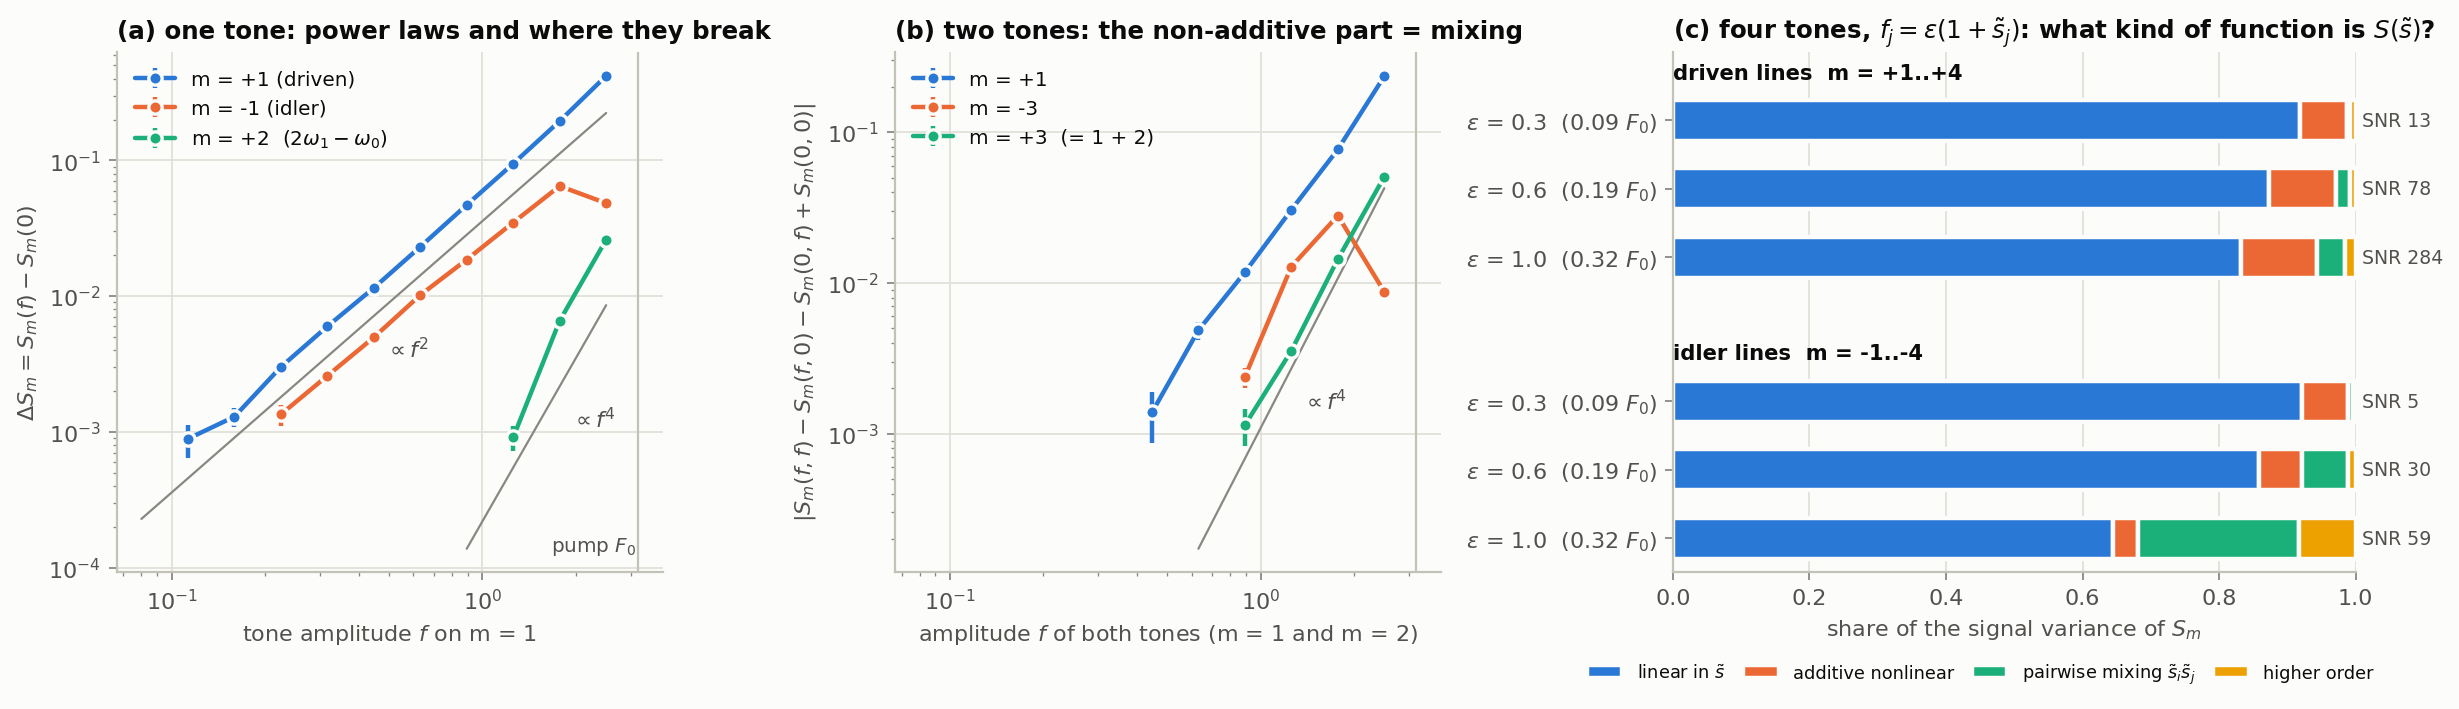
\includegraphics[width=\textwidth]{characterization/02_subband_nonlinearity.png}
\caption{Chaotic comb: how nonlinear is the response to the tones?  (a)~One tone on $m=1$: the driven line and its idler
follow $\propto f^2$ (linear response) up to $f\approx0.8\Fz$; the second-order product $2\omega_1-\omega_0$ appears
$\propto f^4$.  (b)~Two tones: the part of the response that is not the sum of the single-tone responses.  (c)~Four tones
with the actual encoding: variance decomposition of the driven and idler lines.  SNR is the signal-to-chaos-noise ratio of
the $\Tavg=100$ features.}
\label{fig:nonlin}
\end{figure}
\begin{figure}[h]
\centering
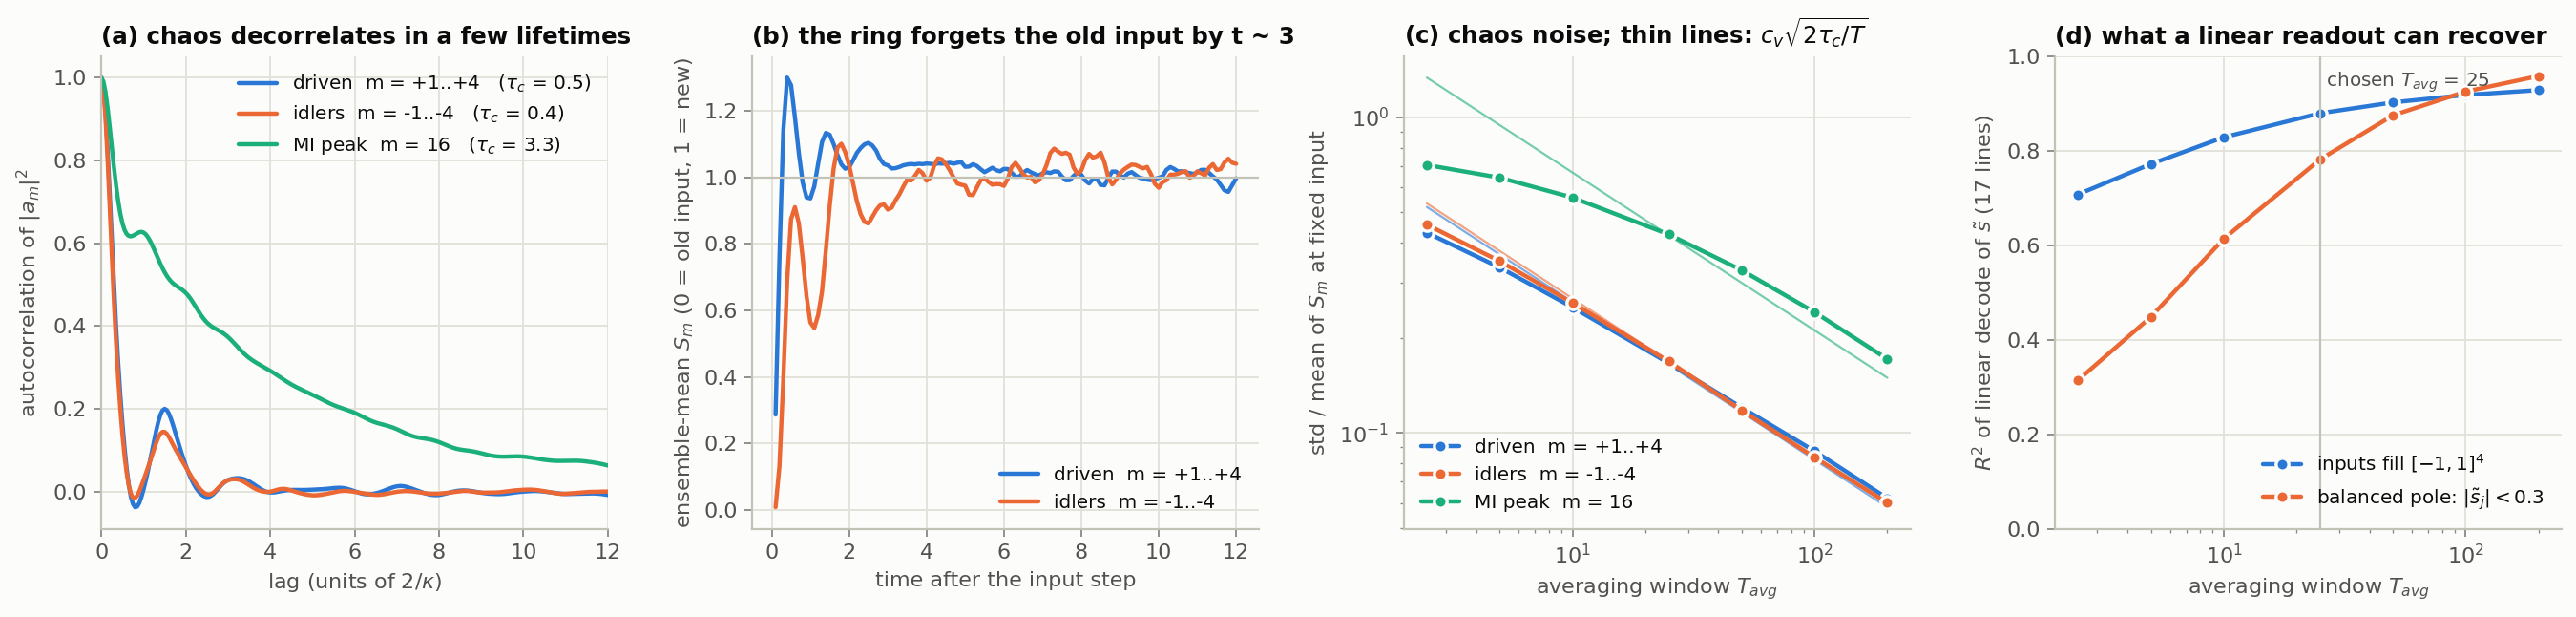
\includegraphics[width=\textwidth]{characterization/03_averaging_window.png}
\caption{Chaotic comb: choosing the averaging window.  (a)~Intensity autocorrelation of the comb lines.  (b)~Ensemble
response to an input step.  (c)~Chaos noise versus window, with the prediction $c_v\sqrt{2\tau_c/T}$.  (d)~Fraction of the
input variance a linear readout of the 17 lines recovers, for inputs filling the cube and for the small excursions of a
balanced pole.}
\label{fig:avg}
\end{figure}
\begin{figure}[h]
\centering
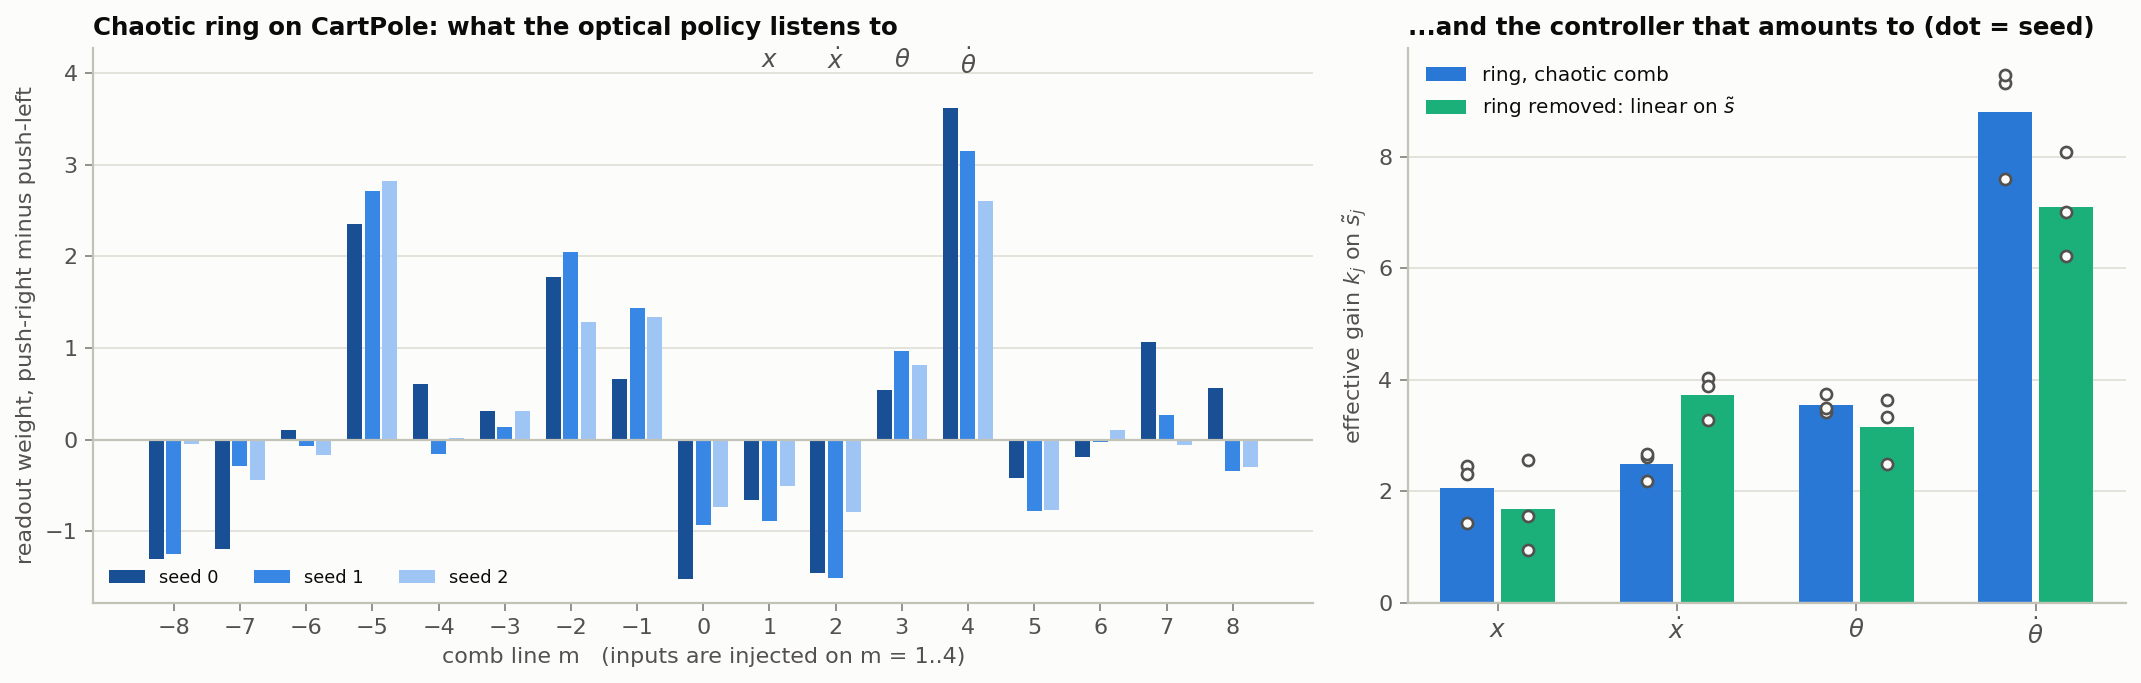
\includegraphics[width=\textwidth]{ppo/CartPole/readout.png}
\caption{The trained chaotic-ring readouts on CartPole.  Left: logit-difference weight on each comb line for three seeds.
Right: the same weights projected through the ring's measured linear response, compared with the gains of the linear policy
trained without the ring.}
\label{fig:readout}
\end{figure}
\begin{figure}[h]
\centering
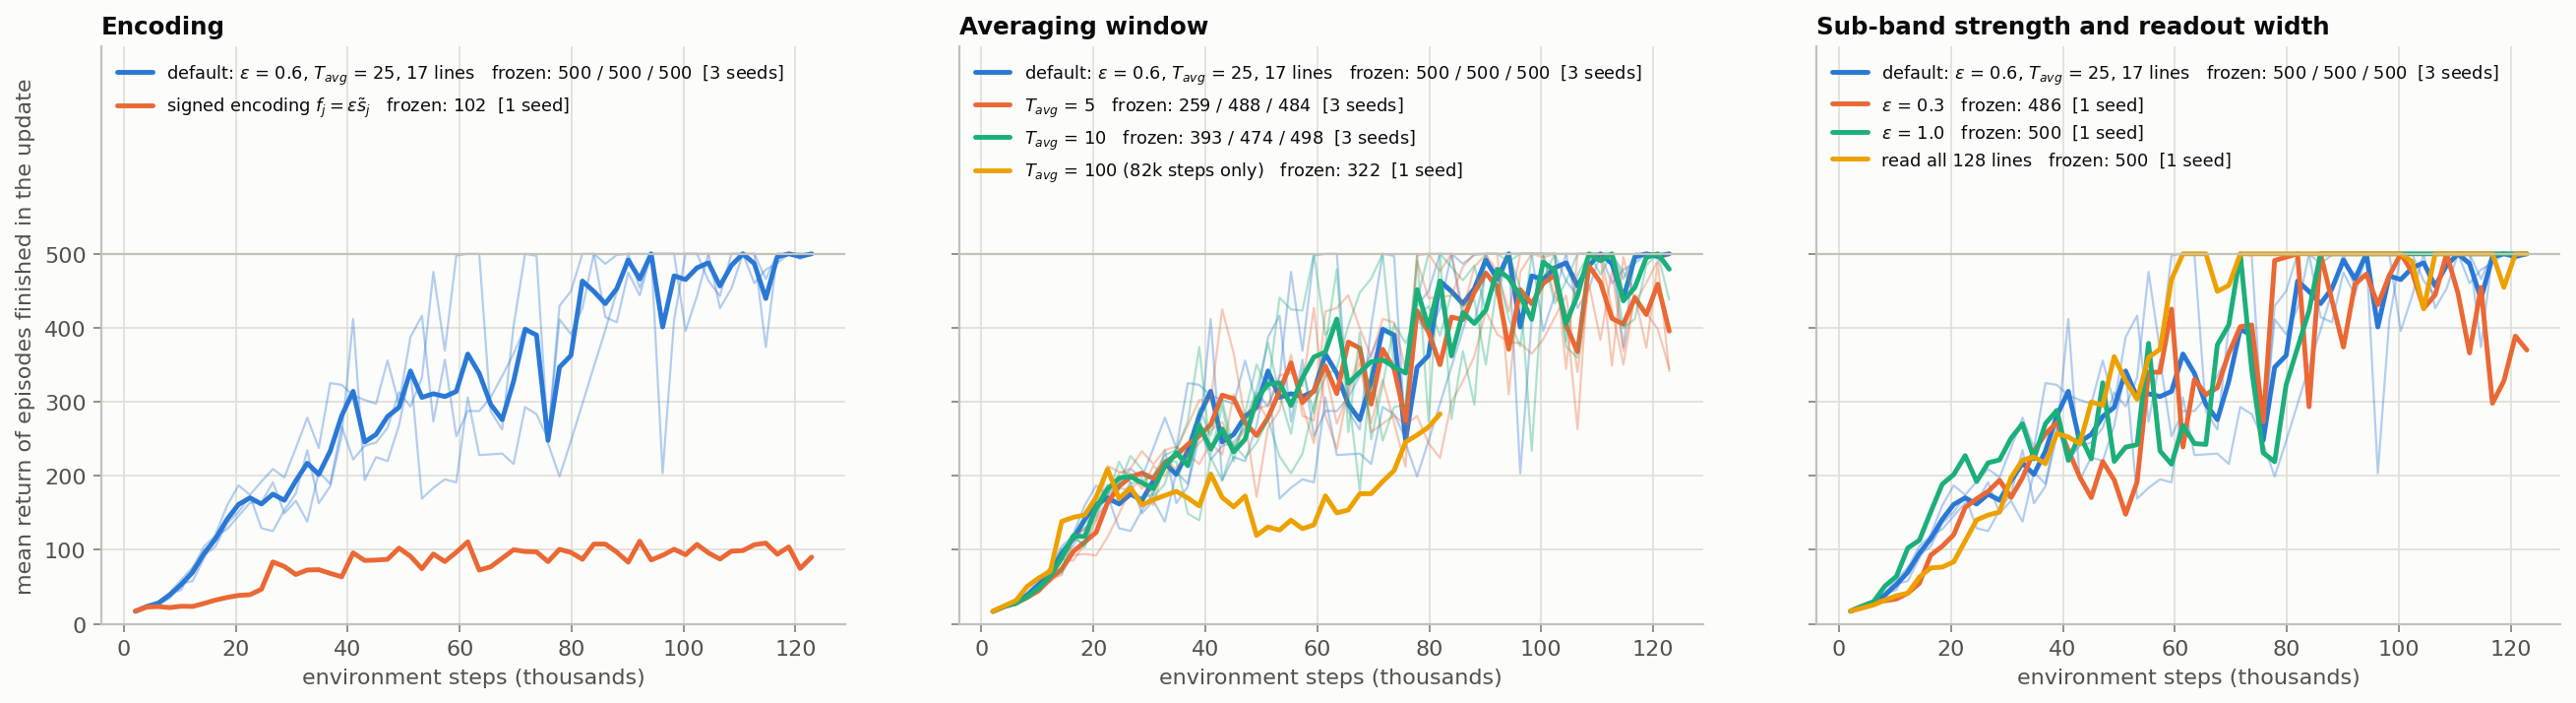
\includegraphics[width=\textwidth]{ppo/CartPole/ablation.png}
\caption{Ablations of the chaotic ring on CartPole (frozen = greedy return of the final policy per seed).}
\label{fig:ablation}
\end{figure}

\begin{thebibliography}{9}\small
\bibitem{ref:sci_rep_2022} K.~Kanno and A.~Uchida, Photonic reinforcement learning based on optoelectronic reservoir computing,
\emph{Sci.\ Rep.} \textbf{12} (2022), doi:10.1038/s41598-022-07404-z.
\bibitem{ref:prr_2025} N.~Shaabani Shishavan \emph{et al.}, Optical neuromorphic computing based on chaotic frequency combs in nonlinear
microresonators, \emph{Phys.\ Rev.\ Research} \textbf{7}, L042008 (2025); reproduced and extended in the companion repository
\texttt{rc-chaotic-comb}.
\bibitem{ref:nanoph_2025} J.~Cuevas, Y.~Hu, B.~Shi, J.~Liu, K.~Minoshima and N.~Kuse, Frequency-multiplexed optical reservoir computing
using a microcomb, \emph{Nanophotonics} (2025), doi:10.1515/nanoph-2025-0260.
\end{thebibliography}

\vspace{4pt}\noindent{\footnotesize Simulations, figures and this note were produced with the assistance of Claude (Anthropic).
All code, run logs and result files are in the repository; every number above can be regenerated with
\texttt{run\_experiments.sh}, \texttt{characterization/} and \texttt{summarize\_results.py}.}
\end{document}
